\section{Example 2 - Image Compression}

Ví dụ này dùng K-means để giảm số màu của ảnh chụp từ webcam. Mỗi điểm ảnh
được xem là một điểm dữ liệu trong không gian màu RGB. Thuật toán gom các
màu gần nhau thành $K$ cụm; khi tái tạo ảnh, màu của mỗi điểm ảnh được thay
bằng màu tâm của cụm tương ứng. Mã nguồn nằm trong tệp
\texttt{k-means-img\_compression.py}.

\subsection{Block 1: Nguyên lý biểu diễn màu}

\textbf{Trước khi giảm màu:} Một điểm ảnh RGB có ba giá trị $R$, $G$, $B$,
mỗi giá trị dùng 8 bit, tức $8+8+8=24$ bit/điểm ảnh. Với ảnh
$640\times480$, lượng dữ liệu màu thô là
\begin{equation}
    640\times480\times24=7\,372\,800\ \text{bit}.
\end{equation}

\textbf{Sau khi giảm màu, minh họa với $K=16$:} Mỗi điểm ảnh chỉ cần một
chỉ số trong tập $\{0,1,2,\ldots,15\}$, nên chỉ số cần 4 bit. Một bảng màu
lưu giá trị RGB ứng với từng chỉ số. Chẳng hạn, bảng màu minh họa ban đầu
có thể viết gọn như sau:
\begin{center}
    \begin{tabular}{cc}
        \toprule
        \textbf{Chỉ số} & \textbf{Giá trị RGB minh họa} \\
        \midrule
        $0$ & $[240,\,50,\,60]$ \\
        $1$ & $[20,\,20,\,20]$ \\
        $2$ & $[180,\,150,\,130]$ \\
        $\vdots$ & $\vdots$ \\
        $15$ & $[90,\,100,\,120]$ \\
        \bottomrule
    \end{tabular}
\end{center}
Nếu lưu ảnh theo dạng chỉ số màu kèm bảng màu, dung lượng lý thuyết cho
$K=16$ là $640\times480\times4+16\times24=1\,229\,184$ bit.

Trong chương trình thực tế, \texttt{K = 20}. Cần 5 bit để mã hóa một trong
20 chỉ số màu, nên dung lượng lý thuyết tương ứng là
\begin{equation}
    640\times480\times5+20\times24=1\,536\,480\ \text{bit}.
\end{equation}
Các phép tính trên mô tả cách lưu ảnh bằng bảng màu. Chương trình xuất ảnh
JPEG, vì vậy dung lượng tệp thực tế còn phụ thuộc cách mã hóa JPEG.

\subsection{Block 2: Chụp ảnh và chuẩn bị dữ liệu}

Hàm \texttt{capture\_from\_webcam} mở webcam, hiển thị đếm ngược 3 giây,
lật khung hình theo chiều ngang rồi lưu ảnh gốc vào
\texttt{webcam\_capture.jpg}. Ảnh do OpenCV đọc có thứ tự kênh BGR; trước
khi xử lý và hiển thị, mã chuyển sang RGB. Khối \texttt{finally} giải phóng
webcam và đóng cửa sổ hiển thị sau khi chụp hoặc gặp lỗi.

\lstinputlisting[
  firstline=9,
  lastline=42,
  firstnumber=9,
  caption={Chụp ảnh từ webcam và chuyển thứ tự kênh BGR sang RGB.},
  label={lst:compression-capture}
]{../src/k-means-img_compression.py}

\lstinputlisting[
  firstline=44,
  lastline=51,
  firstnumber=44,
  caption={Đặt đường dẫn, chụp ảnh gốc và kiểm tra kích thước ảnh.},
  label={lst:compression-original}
]{../src/k-means-img_compression.py}

Ảnh được lưu trong thư mục \texttt{src} có kích thước
$640\times480$ điểm ảnh. Với ảnh RGB có chiều cao $H$, chiều rộng $W$,
lệnh \texttt{reshape} biến mảng ảnh $(H,W,3)$ thành ma trận
$X\in\mathbb{R}^{HW\times3}$. Ở đây $X$ có kích thước $(307\,200,3)$:
mỗi hàng là một điểm ảnh, còn ba cột là ba thành phần màu.

\lstinputlisting[
  firstline=61,
  lastline=75,
  firstnumber=61,
  caption={Chuyển ảnh thành ma trận các điểm màu RGB và chọn $K=20$.},
  label={lst:compression-reshape}
]{../src/k-means-img_compression.py}

\subsection{Block 3: Phân cụm màu bằng K-means}

\texttt{KMeans(n\_clusters=K, random\_state=0)} học 20 tâm màu từ các
hàng của $X$. Mỗi tâm là một bộ ba giá trị RGB đại diện cho một nhóm màu.
Lệnh \texttt{predict(X)} gán cho từng điểm ảnh chỉ số tâm gần nhất; vì $X$
chính là dữ liệu vừa dùng để huấn luyện, mảng nhãn này cũng có thể lấy từ
\texttt{kmeans.labels\_}.

\lstinputlisting[
  firstline=75,
  lastline=88,
  firstnumber=75,
  caption={Huấn luyện K-means và lấy nhãn màu cho từng điểm ảnh.},
  label={lst:compression-kmeans}
]{../src/k-means-img_compression.py}

\subsection{Block 4: Tái tạo và lưu ảnh giảm màu}

Với mỗi cụm $k$, chương trình thay màu của các điểm ảnh có nhãn $k$ bằng
tâm màu $\boldsymbol{\mu}_k$:
\begin{equation}
    \widehat{\mathbf{x}}_i=\boldsymbol{\mu}_{z_i},
    \qquad z_i\in\{0,1,\ldots,19\}.
\end{equation}
Sau đó ma trận màu được đưa về kích thước ảnh ban đầu và lưu thành
\texttt{webcam\_capture\_compressed.jpg}. Trong bộ nhớ, ảnh tái tạo có tối
đa 20 màu khác nhau.

\lstinputlisting[
  firstline=91,
  lastline=103,
  firstnumber=91,
  caption={Thay màu từng điểm ảnh bằng tâm cụm, khôi phục hình dạng và lưu ảnh.},
  label={lst:compression-reconstruct}
]{../src/k-means-img_compression.py}

\subsection{Block 5: Kết quả và nhận xét}

\begin{figure}[htbp]
    \centering
    \begin{subfigure}[t]{0.48\textwidth}
        \centering
        
\includegraphics[width=\linewidth]{../src/webcam_capture.jpg}
        \caption{Ảnh gốc.}
    \end{subfigure}\hfill
    \begin{subfigure}[t]{0.48\textwidth}
        \centering
        
\includegraphics[width=\linewidth]{../src/webcam_capture_compressed.jpg}
        \caption{Ảnh sau K-means với $K=20$.}
    \end{subfigure}
    \caption{So sánh ảnh webcam trước và sau khi giảm số màu.}
    \label{fig:compression-compare}
\end{figure}

Quan sát Hình~\ref{fig:compression-compare}, hình dạng và các vùng màu chính
vẫn được giữ lại, nhưng vùng chuyển sắc và một số chi tiết nhỏ trở nên thô
hơn vì nhiều màu ban đầu cùng được thay bằng một màu đại diện. Hai tệp JPEG
hiện có lần lượt chiếm $85\,480$ và $34\,222$ byte; tệp sau xử lý nhỏ hơn
khoảng $60\%$. Đây là dung lượng tệp JPEG đo được, không phải dung lượng
lý thuyết của cách lưu chỉ số màu ở Block 1.

Mã còn đếm số màu khác nhau của ảnh gốc và ảnh tái tạo trong bộ nhớ bằng
\texttt{np.unique}. Ảnh tái tạo trong bộ nhớ có không quá 20 màu, nhưng tệp
JPEG khi đọc lại có thể chứa nhiều giá trị RGB hơn do quá trình mã hóa ảnh.

\begin{figure}[htbp]
    \centering
    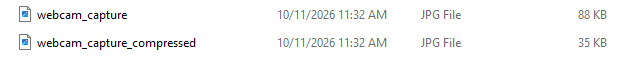
\includegraphics[width=1\textwidth]{../report/images/storage_occupy.png}
    \caption{Kích thước tệp JPEG trước và sau khi giảm số màu.}
    \label{fig:compression-colors}
\end{figure}

\lstinputlisting[
  firstline=110,
  lastline=119,
  firstnumber=110,
  caption={Đếm số màu khác nhau trước và sau khi phân cụm trong bộ nhớ.},
  label={lst:compression-colors}
]{../src/k-means-img_compression.py}

\begin{lstlisting}[
  style=terminaloutput,
  caption={Số màu khác nhau của ảnh gốc và ảnh tái tạo trong bộ nhớ.},
  label={lst:kmeans-terminal}
]
Number of colors in original image: 145484
Number of colors in compressed image: 20
\end{lstlisting}
